\chapter{Συμπεράσματα - Προτάσεις για το μέλλον} \label{ch:conclusion}
\markboth{Συμπεράσματα}{}

Στην ενότητα αυτή παρουσιάζονται συνοπτικά τα πλεονεκτήματα και τα μειονεκτήματα του συστήματος πλοήγησης που προτείνεται στην εργασία μας. Παράλληλα, προτείνονται ορισμένες βελτιώσεις που αφορούν κάποια χαρακτηριστικά του συστήματος με σκοπό την συνολική αύξηση της απόδοσης, αλλά και της χρηστικότητάς του. Στόχος της παρούσας διπλωματικής εργασίας ήταν η υλοποίηση ενός διακριτικού συστήματος πλοήγησης για άτομα με προβλήματα όρασης, το οποίο θα υποβοηθούσε τον χρήστη να διασχίζει τους δρόμους και να μετακινείται με περισσότερη άνεση και ασφάλεια μέσα σε ένα αστικό περιβάλλον με παράλληλη χρήση του λευκού μπαστουνιού. Ο στόχος αυτός επετεύχθη και, παρ' όλες τις ατέλειες του συστήματος, η τελική πειραματική υλοποίησή του είναι λειτουργική και έρχεται πολύ κοντά στις αρχικές φιλοδοξίες του συγγραφέα.

\section{Πλεονεκτήματα}
Το κύριο πλεονέκτημα του συστήματος είναι η ενσωμάτωση διαφορετικών λειτουργιών και η φορητότητά του. Πιο συγκεκριμένα, συνδυάζει τρία επίπεδα καθοδήγησης, την πλοήγηση turn-by-turn, την αποφυγή εμποδίων και την υποβοήθηση διάσχισης διάβασης πεζών. Οι τρεις αυτές λειτουργίες παρέχονται ταυτόχρονα στον χρήστη καθ' όλη την διάρκεια πλοήγησής του. Επιπλέον, το σύστημα χαρακτηρίζεται από διακριτικότητα όσον αφορά τον όγκο του εξοπλισμού που χρησιμοποιεί και ελάχιστη επεμβατικότητα στις συνήθειες και τη συμπεριφορά του χρήστη, καθώς όλα τα μέρη ενσωματώνονται σε ένα τσαντάκι μέσης.

Παράλληλα, η υλοποίηση που προτείνεται είναι αρκετά φιλική προς τον χρήστη και υποστηρίζει την ελάχιστη παρεμβατικότητα, ενώ αξιοποιεί την λογική plug-and-play, δηλαδή ο χρήστης απλά φοράει το τσαντάκι μέσης και ενεργοποιεί το σύστημα μέσω του κινητού του, χωρίς να χρειάζεται περαιτέρω ρύθμιση. Η χρήση των μοτίβων δονήσεων (haptic icons) είναι αρκετά απλή και κατανοητή, μιας και ο αριθμός τους είναι μικρός, μόλις 4 διαφορετικά μοτίβα, και η διαδικασία εκμάθησής τους γρήγορη και εύκολη.

\section{Μειονεκτήματα}
Στα πλαίσια εκπόνησης μιας διπλωματικής εργασίας δεν υπάρχει ο απαραίτητος χρόνος για την υλοποίηση ενός πλήρους και ολοκληρωμένου συστήματος πλοήγησης που θα λειτουργεί απρόσκοπτα χωρίς προβλήματα. Παρόλο, λοιπόν, που το προτεινόμενο σύστημα είναι λειτουργικό, παρουσιάζει όπως είναι φυσικό ορισμένα μειονεκτήματα τα οποία είναι κυρίως αλγοριθμικής φύσεως. Από την άλλη πλευρά, το μοναδικό ίσως μειονέκτημα δομικής φύσεως είναι η χαμηλή απόδοση του συστήματος σε συνθήκες νύχτας, μιας και βασίζεται στην χρήση κάμερας και η ύπαρξη φωτισμού είναι αναγκαία.

\subsection{Ανίχνευση διάβασης πεζών}
Καταρχάς, ο αλγόριθμος ανίχνευσης διάβασης πεζών φαίνεται να είναι επιρρεπής στις περιβαλλοντικές συνθήκες, στις συνθήκες του οδοστρώματος (βρεγμένο ή όχι), ενώ εξαρτάται επίσης και από τον βαθμό συντήρησης της διάβασης πεζών (κατά πόσο έντονη είναι η διαγράμμιση). Μετά από κάποιες δοκιμές, ωστόσο, βρέθηκε ότι η μεγαλύτερη αδυναμία του συγκεκριμένου αλγορίθμου είναι η παραπλάνησή του από εικόνες που περιέχουν σκαλοπάτια, αντί για διάβαση πεζών. Εξαιτίας του γεγονότος ότι αξιοποιείται το εναλλασσόμενο μοτίβο των δύο γραμμών για την αναγνώριση της διάβασης, ο αλγόριθμος βγάζει λάθος συμπεράσματα όταν επεξεργάζεται φωτογραφίες που απεικονίζουν σκαλοπάτια, μιας και οι τελευταίες ενσωματώνουν περίπου το ίδιο εναλλασσόμενο μοτίβο, όπως φαίνεται στο σχήμα \ref{fig:test-zebra4}.

\begin{figure}[H]
    \centering
    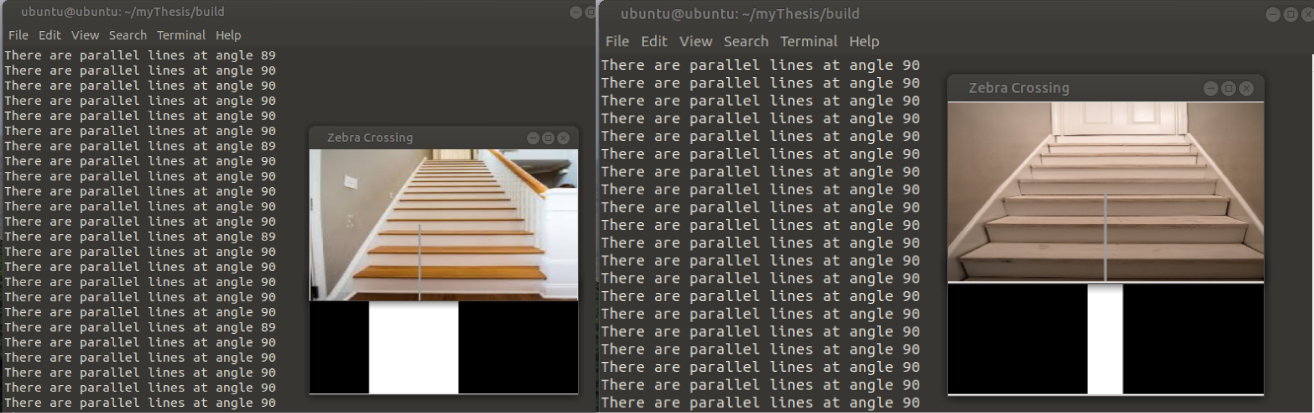
\includegraphics[width=\textwidth]{images/test_zebra4.png}
    \caption{Παράδειγμα παραπλάνησης αλγορίθμου. Το πρόγραμμα αναγνωρίζει λανθασμένα κάποια σκαλοπάτια ως διάβαση πεζών. Αυτό συμβαίνει επειδή τα μοτίβα των σκαλοπατιών και της διάβασης είναι παρόμοια μεταξύ τους.}
    \label{fig:test-zebra4}
\end{figure}

\subsection{Αναγνώριση φωτεινού σηματοδότη}
Όσον αφορά τον αλγόριθμο αναγνώρισης φωτεινού σηματοδότη, η βασική του αδυναμία έγκειται στο γεγονός πως το τελικό αποτέλεσμα εξαρτάται σε πολύ μεγάλο ποσοστό από τον τύπο των templates που χρησιμοποιούνται για την αντιστοίχηση του χρώματος του φαναριού. Τέλος, η φύση του αλγορίθμου αυτού τον καθιστά αρκετά ευάλωτο στις περιβαλλοντικές συνθήκες φωτισμού. Σχετικό παράδειγμα παρουσιάζεται στο σχήμα \ref{fig:test-light5}.

\begin{figure}[H]
    \centering
    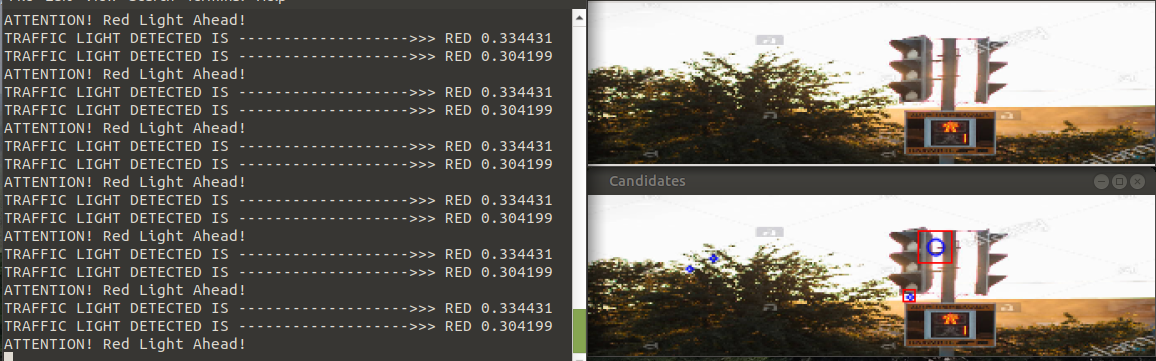
\includegraphics[width=\textwidth]{images/test_light5.png}
    \caption{Παράδειγμα αστοχίας αλγορίθμου. Το πρόγραμμα αναγνωρίζει λανθασμένα κάποια σημεία της εικόνας ως φανάρια και τα ερμηνεύει με κόκκινο χρώμα. Αυτό συμβαίνει επειδή υπάρχουν έντονες αντανακλάσεις του ηλιακού φωτός, ενώ αντίστοιχα η ένταση της φωτεινότητας του φαναριού είναι χαμηλή.}
    \label{fig:test-light5}
\end{figure}

\section{Μελλοντικές προτάσεις}
Οι παρακάτω προτάσεις αφορούν την βελτίωση ορισμένων χαρακτηριστικών του συστήματος τα οποία θα αυξήσουν άμεσα την απόδοση και την αποτελεσματικότητά του και τα οποία δεν μπόρεσαν να υλοποιηθούν, κυρίως, λόγω έλλειψης χρόνου.

\subsection{Μετατροπέας Voice-to-Text}
Μια αναγκαία προσθήκη που απαιτείται για να κάνει το παραπάνω σύστημα πλήρως προσβάσιμο σε άτομα με προβλήματα όρασης είναι η ενσωμάτωση ενός μετατροπέα φωνής σε κείμενο (Voice-to-Text) και, αντίστροφα, κειμένου σε φωνή (Text-to-Voice). Με τον τρόπο αυτό ο χρήστης θα μπορεί να πλοηγείται στην εφαρμογή πλήρως ανεξάρτητα, ενώ η εισαγωγή του προορισμού θα γίνεται μέσω φωνητικών εντολών του χρήστη. Για την υλοποίηση του τελευταίου, υπάρχει ήδη διαθέσιμο Google API για android development που χρησιμοποιεί τον αλγόριθμο αναγνώριση φωνής της Google.

\subsection{Αναγνώριση εμποδίων}
Δεύτερη σημαντική προσθήκη είναι η βελτίωση του υπάρχοντος αλγορίθμου εντοπισμού εμποδίων. Πιο συγκεκριμένα, για να είναι πιο αποδοτικός θα πρέπει να χρησιμοποιεί πιο εξελιγμένη λογική στην ανάλυση της εικόνας βάθους και να ενσωματώνει λειτουργία αναγνώρισης του είδους των εμποδίων που ανιχνεύονται, π.χ. άνθρωπος, κολόνα, αυτοκίνητο κλπ.

\subsection{Βελτιωμένο template φωτεινού σηματοδότη}
Ο αλγόριθμος αναγνώρισης φωτεινού σηματοδότη βασίζεται στην χρήση ενός συγκεκριμένου προτύπου. Ένας τρόπος να αυξήσουμε την απόδοση του αλγορίθμου αυτού είναι να βρεθεί ένα καλύτερο πρότυπο, το οποίο να αντιπροσωπεύει πιο αποτελεσματικά τους φωτεινούς σηματοδότες. Κάτι τέτοιο απαιτεί αντίστοιχη έρευνα για την εξακρίβωση των χαρακτηριστικών εκείνων που παίζουν μεγαλύτερο ρόλο στο template matching.

\subsection{Αυτονομία}
Η αυτονομία ενός συστήματος πλοήγησης είναι ένα από τα κύρια χαρακτηριστικά που ενδιαφέρει τον τελικό χρήστη, καθώς έχει ανάγκη την, όσο το δυνατόν, μεγαλύτερη διάρκεια συνεχόμενης χρήσης.
Η αυτονομία του συστήματος εξαρτάται τόσο από το μέγεθος της φορητής μπαταρίας (powerbank) όσο και από την κατανάλωση του συστήματος. Θεωρώντας δεδομένη την κατανάλωση, θα προτείναμε να γίνει χρήση μιας μεγαλύτερης σε χωρητικότητα μπαταρίας, η οποία θα επιτρέπει την συνεχόμενη χρήση τουλάχιστον 2 ωρών. Για τις ανάγκες της διπλωματικής εργασίας, η αυτονομία της πειραματικής διάταξης ήταν παραπάνω από αρκετή.

\subsection{Usability test}
Τέλος, κάθε σύστημα που προορίζεται για χρήση από τελικούς χρήστες είναι απαραίτητο να περνάει από έναν έλεγχο χρηστικότητας (usability test). Συνήθως ο έλεγχος αυτός περιλαμβάνει την χρήση του προς εξέταση συστήματος από τους πραγματικούς χρήστες, δηλαδή από άτομα που πάσχουν από προβλήματα μειωμένης όρασης, και υπάρχουν διάφορες μέθοδοι που μπορούν να αξιοποιηθούν για τον υπολογισμό μιας μετρικής χρηστικότητας, όπως είναι οι 10 ευρετικοί κανόνες του Nielsen \cite{nielsen1990}.